\section{一般基}
设$\{\bb{g}_1,\bb{g}_2,\bb{g}_3\}$表示任意一组固定的不共面矢量集。那么任意一个矢量$\bb{v}$可以被唯一表示为
\begin{equation}\label{equ:2.1}
    \bb{v}=v^1\bb{g}_1+v^2\bb{g}_2+v^3\bb{g}_3=\sum_1^3{v^i\bb{g}_i}
\end{equation}
如此一来,${\bb{g}_1,\bb{g}_2,\bb{g}_3}$就被称作基底(basis),而它的元素则被称作基矢量。基矢量不需要是单位长度的,也不需要彼此垂直。如图\eqref{fig:2.1}所示便是一个基矢量。

\begin{figure}[htbp]
	\centering
	\begin{minipage}[b]{0.48\textwidth}
        \centering
        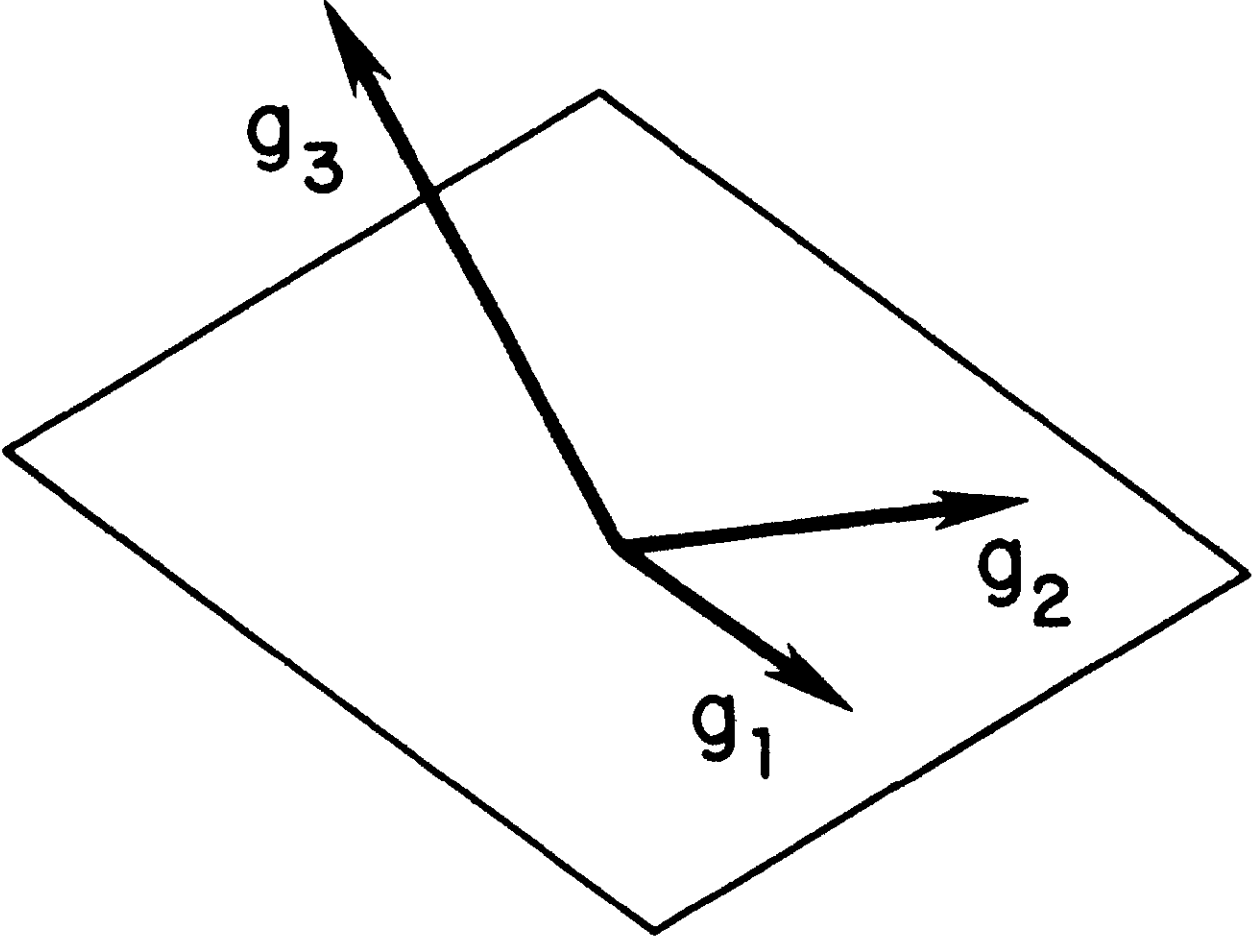
\includegraphics[width=0.85\textwidth]{./image/2.1.png}
        \caption{}
        \label{fig:2.1}
    \end{minipage}
    \begin{minipage}[b]{0.48\textwidth}
        \centering
        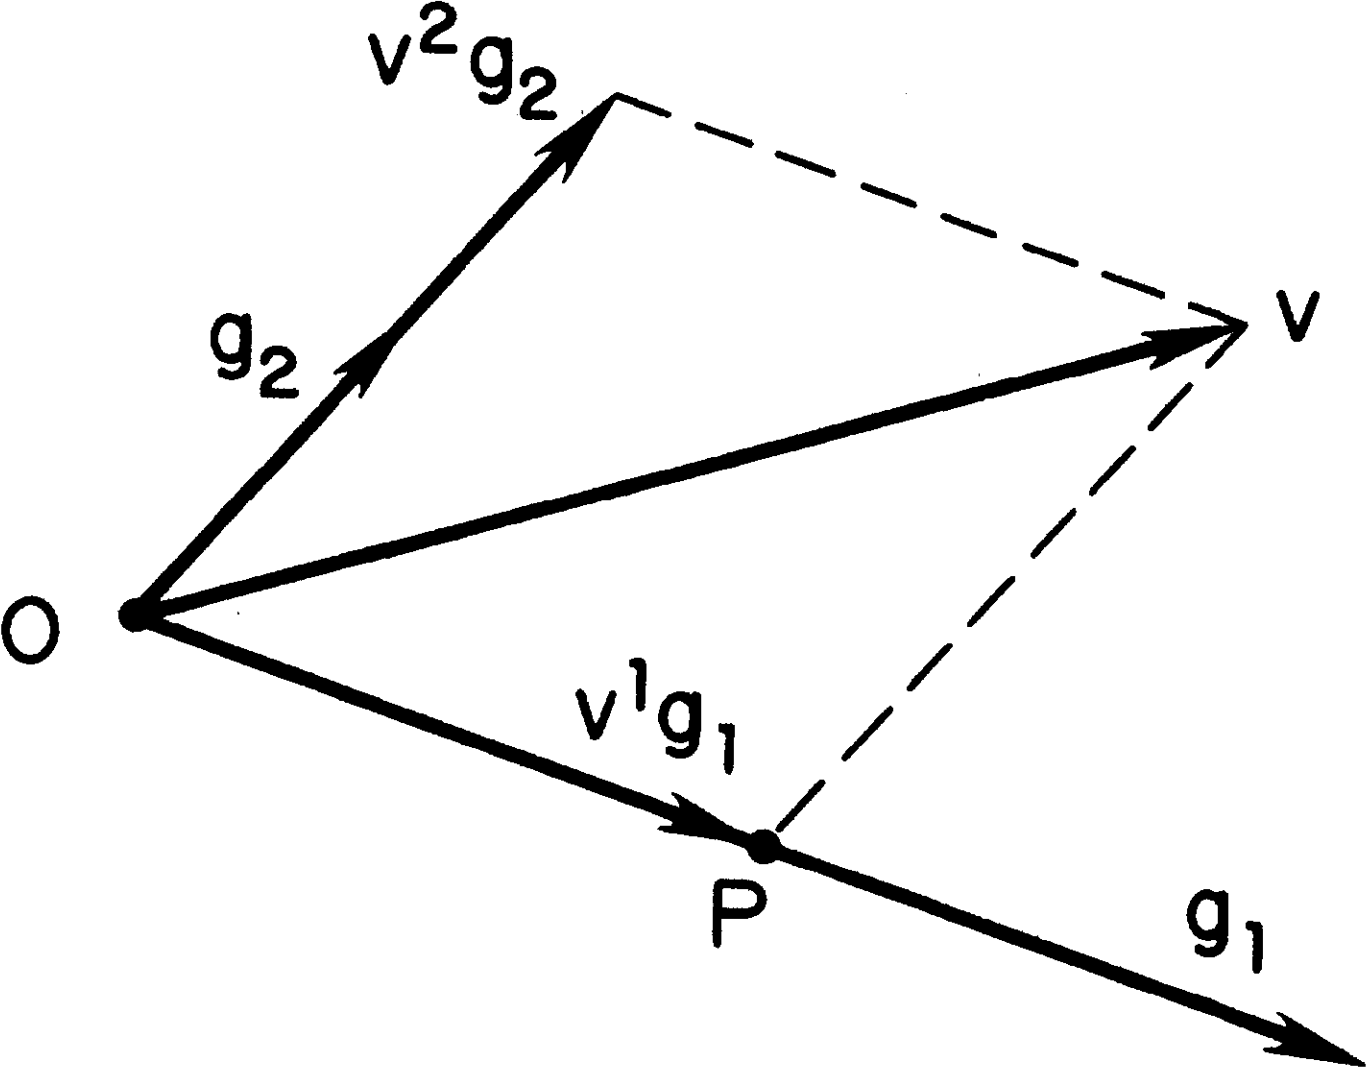
\includegraphics[width=0.85\textwidth]{./image/2.2.png}
        \caption{}
        \label{fig:2.2}
    \end{minipage}
\end{figure}

为了从几何角度理解式\eqref{equ:2.1},我们得先考虑二维情况。在图\eqref{fig:2.2}中,我们绘制一个矢量$\bb{v}$作为代表和一组基底$\left\{ \bb{g}_1,\bb{g}_2 \right\} $,即两个固定的非零不平行矢量。由矢量$\bb{v}$的首端我们引出一条平行于$\bb{g}_2$的线。它与$\bb{g}_1$交于某点$P$。那么,矢量$\rr{OP}$便是某个唯一的标量$v^1$与$\bb{g}_1$的乘积。(所以尽管我们在图中标记的$v^1$是正的,一般情况下,它可正可负。)我们可以用类似的方式构造$v^2$。

在三维情况下,我们同样给出矢量$\bb{v}$和基底$\left\{ \bb{g}_1,\bb{g}_2,\bb{g}_3 \right\} $,所有的矢量都有一个相同的尾端$O$。通过$\bb{v}$的首端,且平行于$\bb{g}_2,\bb{g}_3$所在平面的平面,将与$\bb{g}_1$所在直线交于某点$P$。这便可以确定一个唯一的标量$v^1$使得$v^1\bb{g}_1$为矢量$\rr{OP}$。以同样的方式我们可以确定$v^2$和$v^3$。

表达式\eqref{equ:2.1}可以用如下的方式分析得到。

\begin{example}
    给出
    \begin{equation*}
        \begin{array}{c}
            \bb{g}_1\sim \left( 1,-1,2 \right) ,\bb{g}_2\sim \left( 0,1,1 \right) ,\bb{g}_3\left( -1,-2,1 \right)\\
            \bb{v}\sim \left( 3,3,6 \right)
        \end{array}
    \end{equation*}
    请写出$\left( v^1,v^2,v^3 \right) $。
\end{example}
\begin{solution}
    我们使式\eqref{equ:2.1}两边的笛卡尔坐标相等,即利用式\eqref{equ:1.5} $\sim$式\eqref{equ:1.7},我们可以得到
    \begin{equation*}
        \begin{matrix}
            \begin{aligned}
            3&=\\
            3&=\\
            6&=\\
        \end{aligned}&		\begin{aligned}
            v^1\\
            -v^1\\
            2v^1\\
        \end{aligned}&		\begin{aligned}
            \\
            +v^2\\
            +v^2\\
        \end{aligned}&		\begin{aligned}
            -v^3\\
            -2v^3\\
            +v^3\\
        \end{aligned}\\
        \end{matrix}
    \end{equation*}
    联立求解线性方程组可以得到
    \begin{equation*}
        \left( v^1,v^2,v^3 \right) =\left( 2,3,-1 \right) 
    \end{equation*}
\end{solution}